\clearpage
\lhead{\emph{Chapter 3: The effects of radiation in silicon detectors}}  % Set the left side page header to "Symbols"
\chapter{The effects of radiation in silicon detectors}% No definitivo
\label{chap:rad}
% I haven't talked about leakage current and I most certainly should

When a particle goes through a silicon detector, it can loose energy via ionisation, which is a reversible process because the electrons extracted from the atoms will end up recombining in the material or going back to their original energy level via de-excitation. The impinging particle can also lose energy via non-ionising interactions, where the particle interacts with the Silicon atoms or with the dopant atoms. The effect is detrimental for the detector and leads to a reduction of the collected charge, amongst other macroscopical effects. It is important to understand these changes and have a parametrisation of the degradation. Understanding these defects is fundamental for designing radiation-hard detectors.

In this chapter we summarise the most important mechanisms of radiation damage. One of the key points of the project was to implement radiation damage on the TRACS simulator.


\section{Damaging the lattice}% No definitivo

\begin{figure}[H]
	\centering
	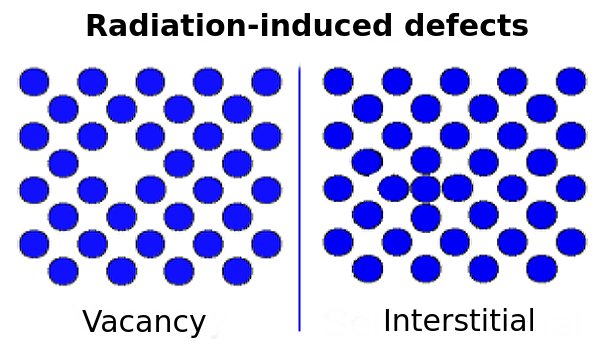
\includegraphics[width=0.8\textwidth]{chap3_defects.png}
	\caption{Interstitial (right) and Vacancy (left) lattice defects are illustrated here. These defects are be created inside silicon detectors after irradiation.}
	\label{fig:IV}
\end{figure}

When a particle transversing the silicon bulk undergoes a non-ionising interaction one or more atoms get knocked-out from their equilibrium position in the lattice, disrupting the ordered structure of silicon. If the atom does not return to the equilibrium position, and Interstitial-Vacancy (I-V) defect is created. The term Interstitial refers to the knocked-off atom misplaced in the lattice and the Vacancy refers to the empty place that it leaves behind as shown in Figure \ref{fig:IV}. This type of defect alters the ordered structure of the lattice and creates a new energy level. The mechanisms by which the I-V defects degrade the performance of the detector and its practical consequences will be discussed in the next sections.

An impinging particle (or the recoil energy of the primarily knocked-off particle) can also create a cluster of defects. The size and clustering of the defects depends on the energy and type of radiation. 

For example, according to \cite{MMoll}, photons with up to 1 MeV energies will create only point defects and no clusters. Electrons can create both point defects and clusters, the latter only occurring for electron energies above 8 MeV. Neutrons will create mainly clusters starting at energies as low as 35keV. 

Typically the NIEL (Non-Ionising Energy Loss) hypothesis is used to characterise the radiation damage caused by any type of particle. The NIEL hypothesis states that the damage produced by radiation of any kind of particle is proportional to the damage produced by 1 MeV neutrons. Therefore fluence of any type of radiation is rescaled to the equivalent fluence of 1MeV neutrons. %the standard unit of measuring the radiation that a silicon detector has undergone is the neutron equivalent (neq).

The I-V defects induced by radiation are not necessarily static defects and their size and configuration varies with temperature in time. For instance, the depletion voltage first decreases with time at a fixed temperature (so-called beneficial annealing) to increase linearly afterwards (long term annealing). Annealing depends heavily on temperature. Defect dynamics observed after 21h at 60C can be slowed down to about 500 years just by cooling down the irradiated detector to -10C \cite{MMollPHD}

\section{Trapping effects} % No definitivo
\label{sec:trapEfect}

The defects induced by radiation affect the drift and collection of the $e-h$ pairs. The I-V defects can create so called $deep-levels$ that can trap and hold charge carriers for times longer than the typical collection times in silicon detectors. The result is a net loss in charge collection efficiency as well as a modified \neff profile.

\begin{figure}[H]
	\centering
	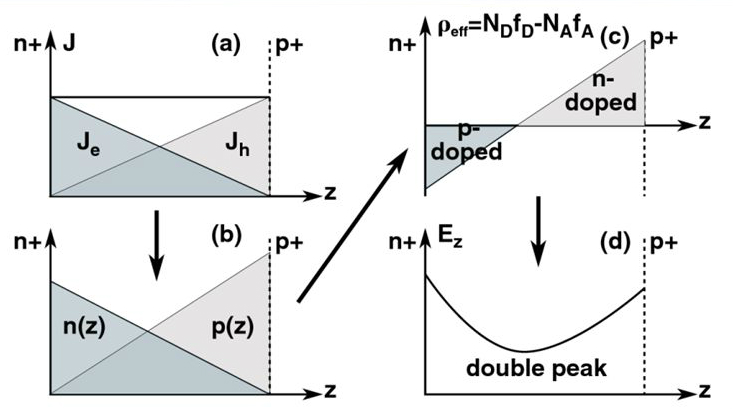
\includegraphics[width=0.8\textwidth]{chap3_erem.jpg}
	\caption{Explanation of the double peak origin is shown in this three schematic plots. $a)$ The carrier current is shown for an diode as being proportional to depth. $b)$ For evenly distributed trapping centres the number of trapped carriers is proportional to their current as shown in $a)$. $c)$ The electric field arising from carrier configuration shown in $b)$ is plotted, the double peak feature becomes now apparent.}
	\label{fig:Eremin}
\end{figure}

To explain why the \neff gets modified after irradiation, we will follow the argument presented by V.Eremin\cite{Eremin}. The current density of $e$ or $h$ ($j_i(z)$), in a fully depleted silicon detector, is not a constant but has a linear dependence with thickness ($z$), as shown  in figure \ref{fig:Eremin}\emph{a}. The concentration of carriers ($n_i(z)$) is proportional to the current $j_i(z)$, so $n_i(z)$ is also linear with $z$. After enough radiation the defects and their correspondent deep levels can be considered uniformly distributed throughout the detector. Then more electrons will be trapped close to the n+ side, and more holes close to the p+ side, simply because the concentration of these carriers is higher there. As a consequence a net negative space charge appears near the n+ side and positive near the p+ side, leading to a \neff profile linear in depth (see Figure \ref{fig:Eremin}\emph{b}). For a more complete description of this argumentation and its validity the reader is referred to \cite{Eremin}.


% Consecuences of a modified Neff (leakage current, higher Vdep, type inversion, DP & DJ)

One of the consequences of having a non-constant \neff configuration is that the resulting electric field inside the detector gets modified. In the linear case a parabolic electric field appears (see Figure \ref{fig:Eremin}\emph{c}) giving rise to a characteristic \emph{double peak} (DP) shape of the transient waveforms. Another consequence of not having a constant \neff is the appearance of a second $p-n$ junction at the end of the detector creating the double junction (DJ) effect. The existence of the DJ means that in a non-fully depleted detector both ends remain sensitive to radiation.

%Other effects of the modified \neff of lesser importance for this project are the increase in leakage current, a higher \vias needed for depleting the full detector volumen, and more exotic processes such as type inversion. % Deberia hablar algo mas de type inversion? decir lo que es?

% EXPLAIN WHY IT MIGHT NOT BE LINEAR but something more exotic (link with TRACS capabilities)

So far it has only been considered that the modification of the \neff due to radiation-induced defects gives rise to a linear \neff inside the detector. However, this might not be always the case, as it has been proposed in more recent publications\cite{KramVertex}. Analysis performed using edge-TCT (see \ref{sec:eTCT} techniques suggest that the \neff configuration might have three different regions in which \neff value is different. This parametrisation will be referred to as \emph{triconstant} and can also explain the DJ and DP effects seen experimentally. As it will be explained in detail later, both linear and triconstant parametrisations have been implemented into TRACS as well as a third parametrisation consisting of three linear regions.  

Besides altering the space charge profile, deep levels induced by radiation have also an impact on signal collected. When charge carriers drift through the irradiated volume they may get trapped in a radiation-induced defect and may remain there for as long as several miliseconds. This is much longer than the collection time of the electronics (of the order of tens of nanoseconds) so they are effectively lost for the electronics. As a result, the waveform shape gets distorted (as it will be explained in the following section) and the charge collected decreases worsening the performance of the detector.

\section{Signal degradation} % No definitivo
\label{sec:signalDeg}

%After taking a look at the effects that radiation has on silicon it is important to understand how radiations changes the read-out signal, since that is what will be measured in the laboratory. As we have already mentioned the main effect of radiation damage from a practical point of view is the creation of deep levels inside the band gap that act as trapping centers for the charge carriers moving inside the silicon bulk. For the sake of simplicity and ease of explanation when explanation when talking about the implementation of radiation damage in the software TRACS, we will treat \neff deformation as a different effect. This is very practical as it helps understand dynamical and static effects separately. 

%The effect that deep levels have in the signal is the trapping of the charge carriers creating a loss in charge collection efficiency. Because collection times in silicon detectors are of the order of tens of nanoseconds whilst the trapping times are typically of the order of milliseconds, the trapped carriers will never be released in time to be collected and are effectively lost. The process of trapping is a statistical one with the probability of one charge carrier to be trapped after a drifting inside the silicon for a time $t$ being  \[FORMULA FOR TRAPPING PROBS\] where $\tau$ (trapping time) is an experimentally determined parameter that shows how likely it is for a carrier to get trapped, in a very similar law as that governing the natural decay of radioactive materials. For a big enough number of carriers drifting in silicon, the effective result in the signal generated is an exponential decrease over time in the collected signal with respect to the unirradiated case. 

%On the other hand the \neff modification due to radiation has no effect on the total collected charge, but on the shape of the collected signal as well as in the collection time. As discussed before the intensity recorded is proportional to the electric field in which the carriers are drifting. Since the electric field is obtained by integrating the \neff, this field is now modified by radiation and yields different waveforms when measured in the lab. Since velocity is different from the non-irradiated case, collection times are modified becoming larger after irradiation in most cases due to lower electric field modulus in the middle of the bulk of silicon. 

%Both effects combined yield the typical $double peak$ shape obtained when subjecting the irradiated detectors to the TCT analysis that are normally performed in the lab. This shape combines the double peak feature of the electric field with the exponential dampening of the electrical charge collected. This kind of measurements and analysis are very useful in studying the charateristics of irradiated silicon detectors including determination of trapping times, \neff profile and charge collection efficiency, as it will be shown in the following chapter.

The effects of radiation in detector performance can be observed both in terms of the total collected charge and the shape of the transient waveforms. The modified \neff distribution inside the detector has an effect on the shape of the waveforms while the effects of trapping centres can be seen both in the waveforms duration and amplitude and also in the total collected charge.

It has been explained in section \ref{sec:Ramo} that the  $ I (t) $ profile of the collected signal from the detector depends on the $\overrightarrow E $ inside of it. It then follows that a modified \neff  (and consequently a modified  $\overrightarrow E$ ) will have an effect in the collected signal and might show a double peak (DP) due to the previously mentioned DJ effect. The collection time might also be affected for the same reason.

For the trapping effects, the probability that a carrier drifting inside the silicon gets trapped in the radiation-induced deep levels after a time $dt$ is

\[p_{trap} = 1/\lambda \cdot dt\] % Need to check bibliography

with $\lambda$ the effective carrier trapping distance that can be different for electrons and holes. We will use $\tau \approx \frac{\lambda}{v_{th}}$ with $\tau$ being the trapping time and $v_{th}$ the thermal velocity of the carrier and can be used in most situations\cite{Kramberger} since $v_{th} > v_{drift}$. $\tau$ is an experimentally determined parameter that is usually taken to be constant or dependant on the electric field and type of carrier.For the rest of the report we will consider $\tau$ to be a constant except otherwise stated. This allows to write the number of non trapped carriers $N$ after drifting in the detector for a time $\Delta t$ as [\cite{Kramberger}, pag 17]

\[N = N_0 \cdot \exp{\big(\frac{-\Delta t}{\tau}} \big)\]

where $N_0 = N(\Delta t = 0)$ the initial number of carriers generated in the detector. Since the intensity is the sum of every carrier's contribution, if we assume that every carrier contributes equally to the total current the previous equation can be re-written as

\begin{equation}
	I(t) = I_0(t) \cdot \exp{\big(\frac{-\Delta t}{\tau}\big)}
 \label{eq:trapCurr}
\end{equation}

where $ I_{0}(t)$ is the current if there were no trapped carriers. 
